\begin{enumerate}
    \item Se desarrolla  en lenguaje C una s-Function  que implementa un filtro Notch con estructura Biquad basado en la estructura entregada como recurso para el laboratorio que se muestra a continuación
    
    \begin{lstlisting}[language = C]
    typedef struct bqState_t {
    double bqA1;
    double bqA2;
    double bqB0;
    double bqB1;
    double bqB2;
    double bqInput[3];
    double bqOutput[3];
} bqState_t;

    \end{lstlisting}
    
    Esta estructura contiene los coeficientes de los polinomios A y B de la función de transferencia de un filtro Biquad de la forma 
    
    $$H(z) = \frac{B(z)}{H(z)} = \frac{b_0 + b_1 z^{1} + b_2 z^{-2}}{1 + a_1 z^{1} + a_2 z^{-2}} $$
    
    
    
    Como lo que se desea implementar es un filtro de tipo Notch, la función de transferencia toma la forma 
    
    \begin{equation}
    H_{BSF} = \frac{1-d}{2} ~ \left  \frac{1 -z^{-1}}{1 - (1+d)cos(\theta) z^{-1} + d^{-z}} \right  \label{p6_Transfer}
    \end{equation}
    
    
    Donde los parámetros $\theta = \frac{2\pi~ f_0}{f_s}$, siendo $f_0$ la frecuencia central de la banda que se desea suprimir con el filtro y $f_s$ la frecuencia de muestreo de la señal que se pretende filtrar.
    
    El parámetro $d$ es el parámetro que permite ajustar el ancho de banda $B_w$ del filtro con la relación 
    
    \begin{equation}
        cos(B_w)d^2 - 2~d + cos(B_w) = 0 \label{p4_cuadratica}
    \end{equation}
     
     Donde $B_w$ corresponde al ancho de banda normalizado con la relación $$B_w = \frac{2\pi ~ (f_{c2}- f_{c1})}{f_s}$$
     Al resolver esta ecuación cuadrática en función del ancho de banda que se desea, obtienen dos raíces del polinomio y se debe escoger aquella que se encuentre dentro del circulo unitario para mantener la estabilidad del sistema ( $|d| < 1$).
     
     
     
     
     Con estas relaciones y considerando $f_0 = 440$, un ancho de banda de $100~Hz$ y $fs = 16 ~kHz$ se pueden calcular los coeficientes para el filtro Notch para filtrar el archivo de audio \textit{alternate\_tones\_16\_16.wav}. Se tiene entonces que 
     
     
     $$ \theta = \frac{2\pi \cdot440~Hz}{16000~Hz} = 0.172787 $$
     
     Y por otro lado 
      $$B_w = \frac{2\pi ~ 100~Hz}{16000~Hz}  = 0.0392699 \Rightarrow d = 0.9614814516$$
     
     $$ a_0 = 1$$
     $$a_1 = -(1-d)cos(\theta) = -1.9322 $$
     $$ a_2 = d =  0.9614814516 $$
     $$ b_0 = \frac{1+d}{2} = 0.9807407258 $$
     $$ b_1 = -2cos(\theta)\cdot \frac{1+d}{2} =  -1.932273671$$
     $$ b_2 = \frac{1+d}{2} = 0.9807407258  $$
     
     Ya con estos coeficientes se puede definir la estructura asociada a este filtro
     
     \begin{lstlisting}[language = C]
        bqState_t Notch440 = {
                      -1.932273671,  // a1
                      0.9614814516, // a2
                      0.9807407258, //b0
                      -1.932273671, //b1
                      0.9807407258,  //b2

                      {0 ,0 ,0}, //Inputs buffer
                      {0,0,0} //Outputs buffer
                    };



     \end{lstlisting}
     
     
    La función que ejecuta el filtrado de la señal haciendo uso del filtro diseñado se implementó con el codigo que se muestra a continuación
    
    \begin{lstlisting}[language = C]
static double filterBiquad(bqState_t *filterNState,
                            double filterInput){
      
//Desplazamiento de datos en la linea de retardo de tamaño 3
filterNState->bqInput[2] = filterNState->bqInput[1];
filterNState->bqInput[1] = filterNState->bqInput[0];
filterNState->bqInput[0] = filterInput;
    
filterNState->bqOutput[2] = filterNState->bqOutput[1];
filterNState->bqOutput[1] = filterNState->bqOutput[0];
    
//y[n] = -a1*y[n] -a2*y[n-2] + b0*x[n] + b1*x[n-1] + b2*x[n-2]
    
double w =  filterNState->bqB0*filterNState->bqInput[0]
            + filterNState->bqB1*filterNState->bqInput[1]
            + filterNState->bqB2*filterNState->bqInput[2];
    
double y = w
        - filterNState->bqA1*filterNState->bqOutput[1]
        - filterNState->bqA2*filterNState->bqOutput[2];
    
filterNState->bqOutput[0] = y;
return y;
}
    \end{lstlisting}
    
    
Y el llamado a dicha función para poder filtrar

\begin{lstlisting}[language = C]
extern double notch(double data){
    return filterBiquad(&Notch440 , data);
}
\end{lstlisting}

Al aplicar el filtro diseñado a la señal de audio \textit{alternate\_tones\_16\_16.wav} y graficar la salida en el tiempo se obtiene la gráfica presente en la figura \ref{alternate100}

\begin{figure}[H]
    \centering
    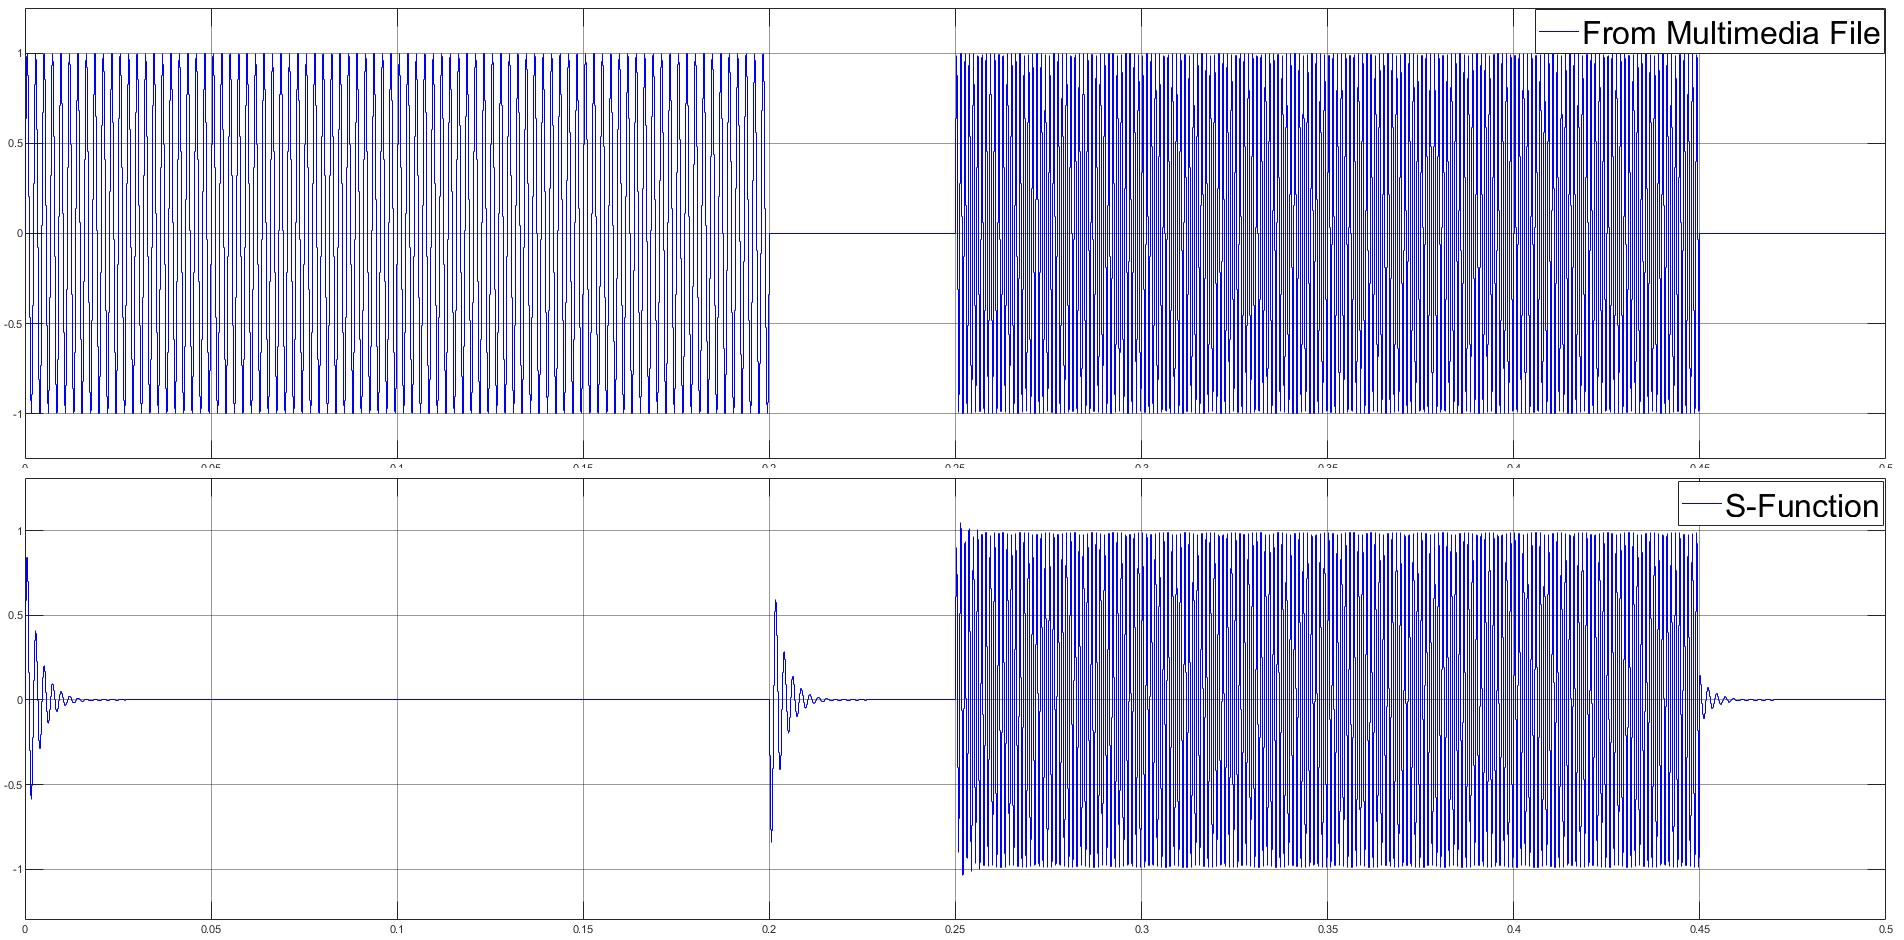
\includegraphics[scale = 0.2]{Figuras/p6_1- alternate_tones_bw100.jpg}
    \caption{Gráfica  en el tiempo de la señal de audio \textit{alternate\_tones\_16\_16.wav} antes y después de ser filtrada con ancho de banda de $100~Hz$}
    \label{alternate100}
\end{figure}



Se diseñan nuevos filtros Notch que realicen la misma tarea pero esta vez con un ancho de banda de $50~Hz$ y $200~Hz$ respectivamente, los resultados obtenidos se muestran en las figuras  \ref{bw50} y \ref{bw200}


\begin{figure}[H]
    \centering
    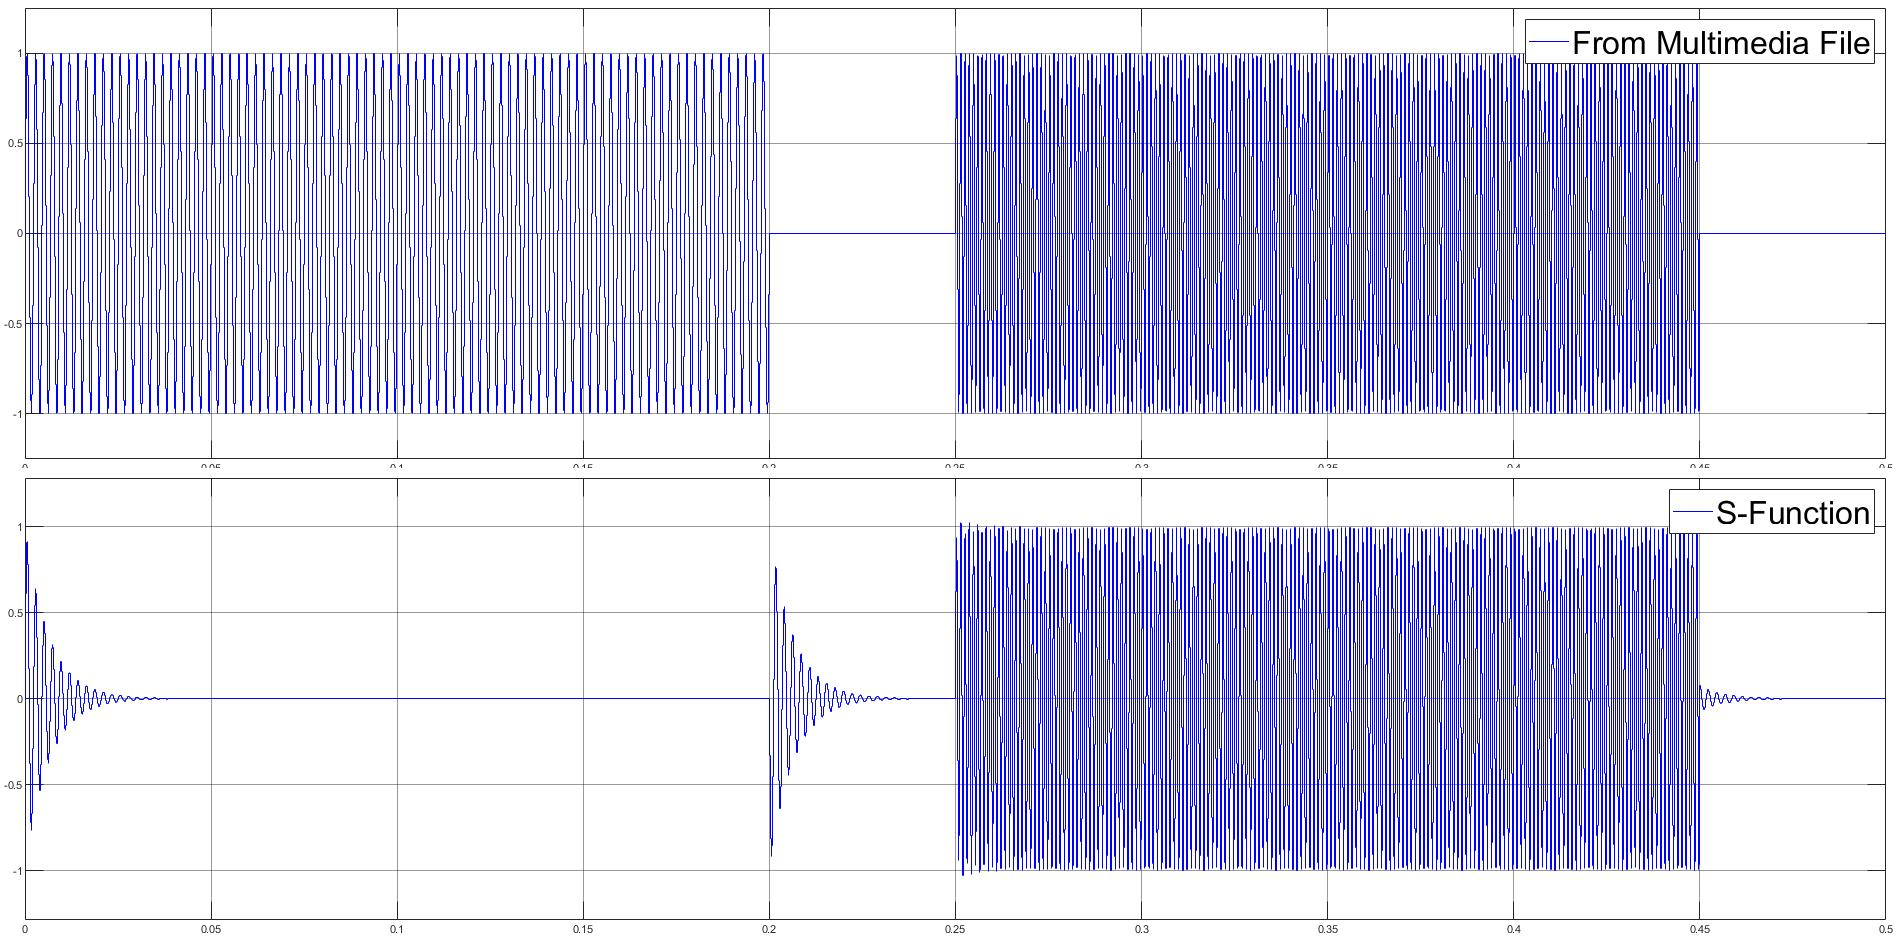
\includegraphics[scale = 0.2]{Figuras/p6_1- alternate_tones_bw50.jpg}
    \caption{Gráfica  en el tiempo en segundos de la señal de audio \textit{alternate\_tones\_16\_16.wav} antes y después de ser filtrada con ancho de banda de $50~Hz$}
    \label{bw50}
\end{figure}


\begin{figure}[H]
    \centering
    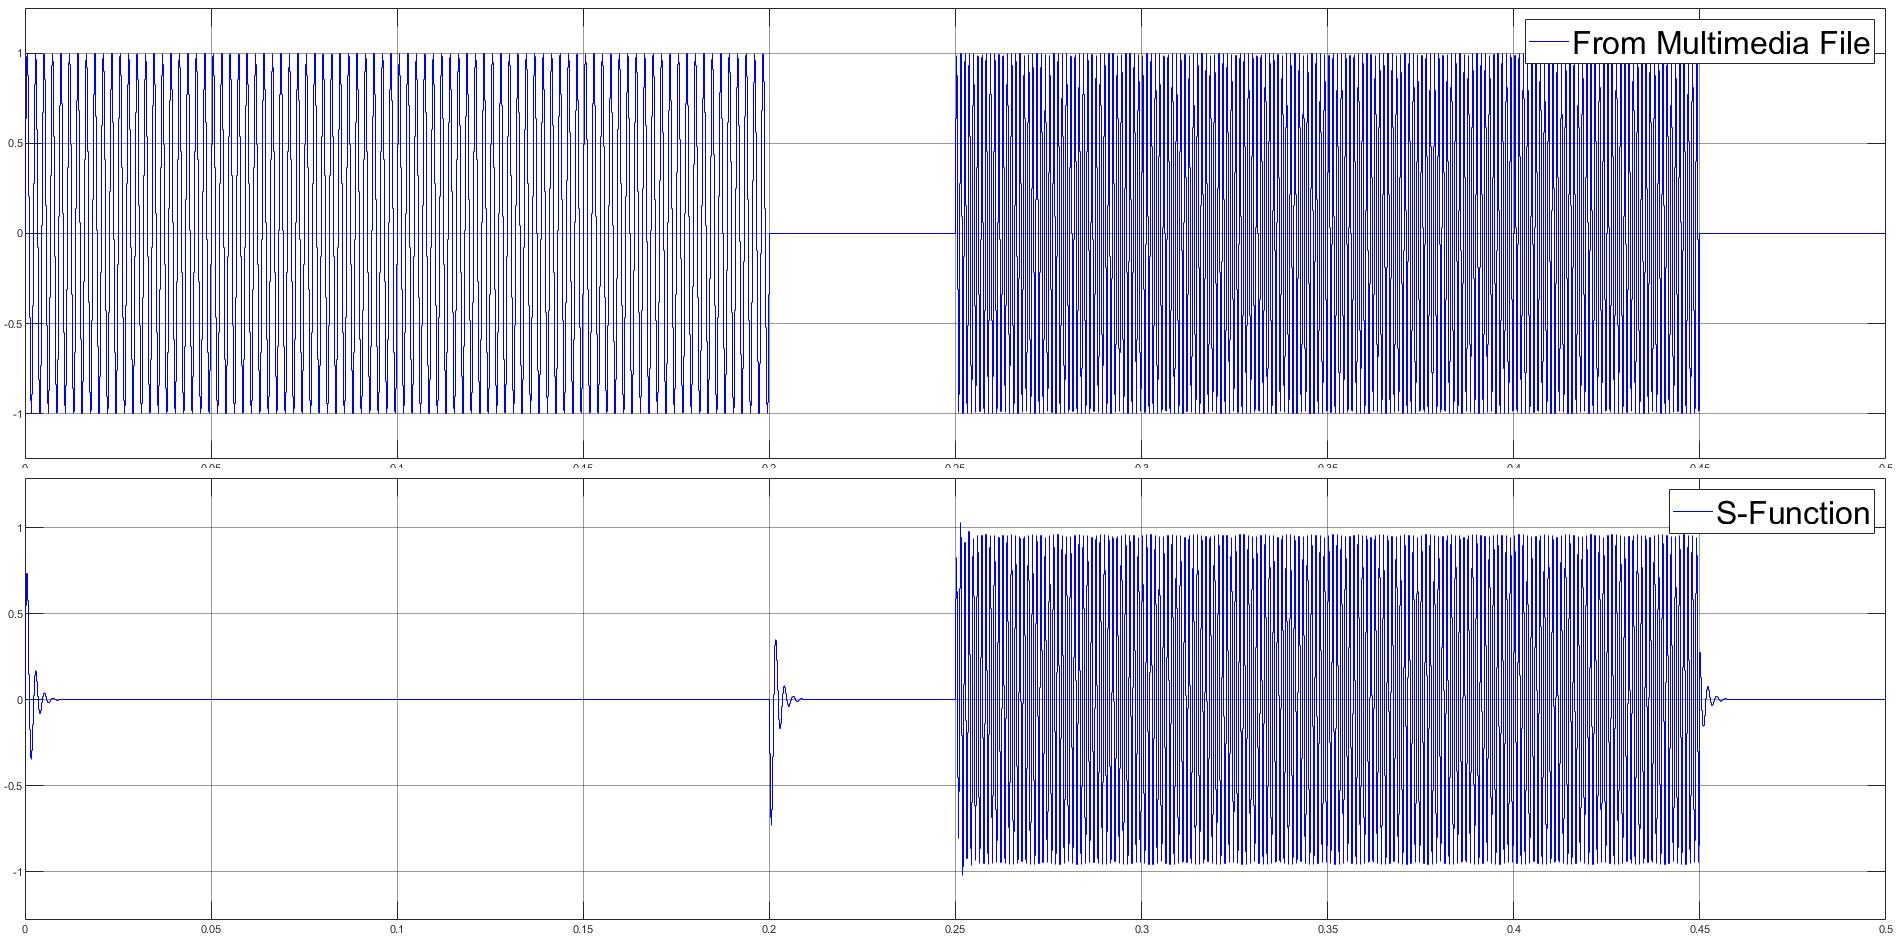
\includegraphics[scale = 0.2]{Figuras/p6_1- alternate_tones_bw200.jpg}
    \caption{Gráfica  en el tiempo en segundos de la señal de audio \textit{alternate\_tones\_16\_16.wav} antes y después de ser filtrada con ancho de banda de $200~Hz$}
    \label{bw200}
\end{figure}


Se puede observar como en todos los casos existe un transciente antes de que se realice efectivamente el filtrado, se concluir por las pruebas realizadas que dicho transciente tiene menor duración en la medida en que aumenta el ancho de banda del filtro. Esto se puede ver de mejor manera observando la respuesta a impulso de los tres filtros diseñados, las respuestas a impulso se encuentran en las figuras \ref{impbw50}, \ref{impbw100} y \ref{impbw200} para los anchos de banda de $50~Hz$, $100~Hz$ y $200~Hz$ respectivamente.

\begin{figure}[H]
    \centering
    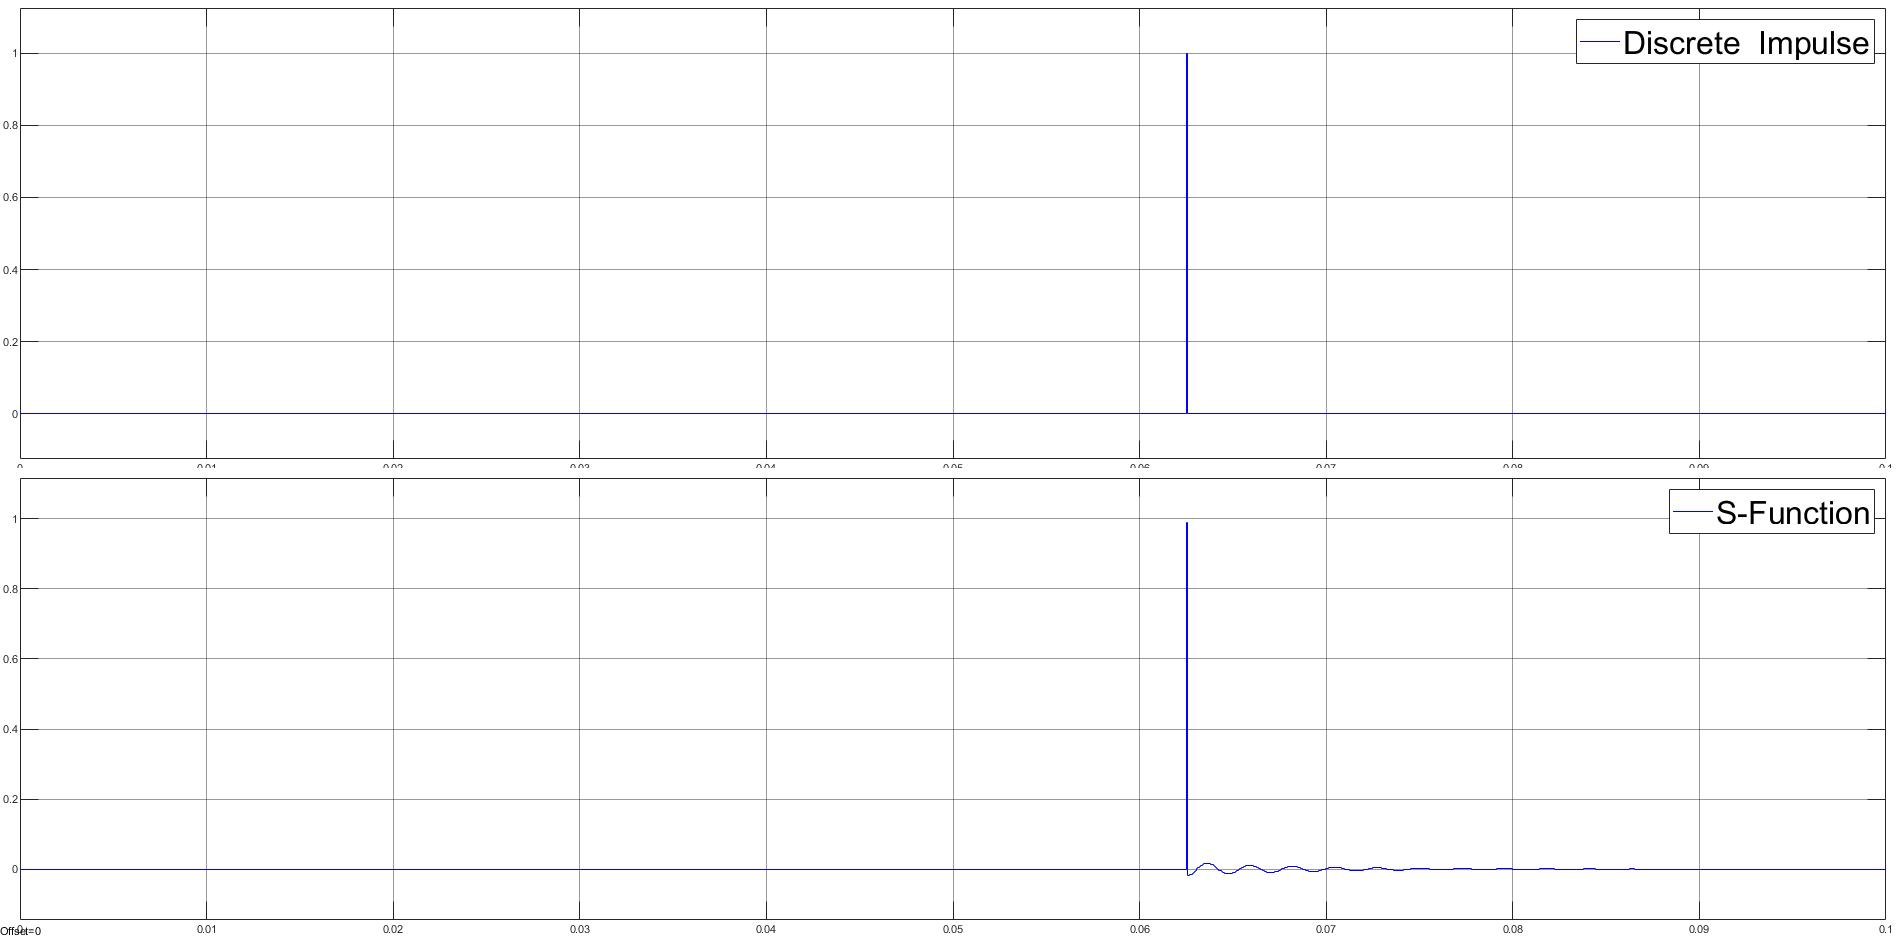
\includegraphics[scale = 0.2]{Figuras/p6_1-Impulse_50.jpg}
    \caption{Gráfica en el tiempo en segundos  de la respuesta impulso del filtro diseñado con ancho de banda de $50~Hz$.}
    \label{impbw50}
\end{figure}


\begin{figure}[H]
    \centering
    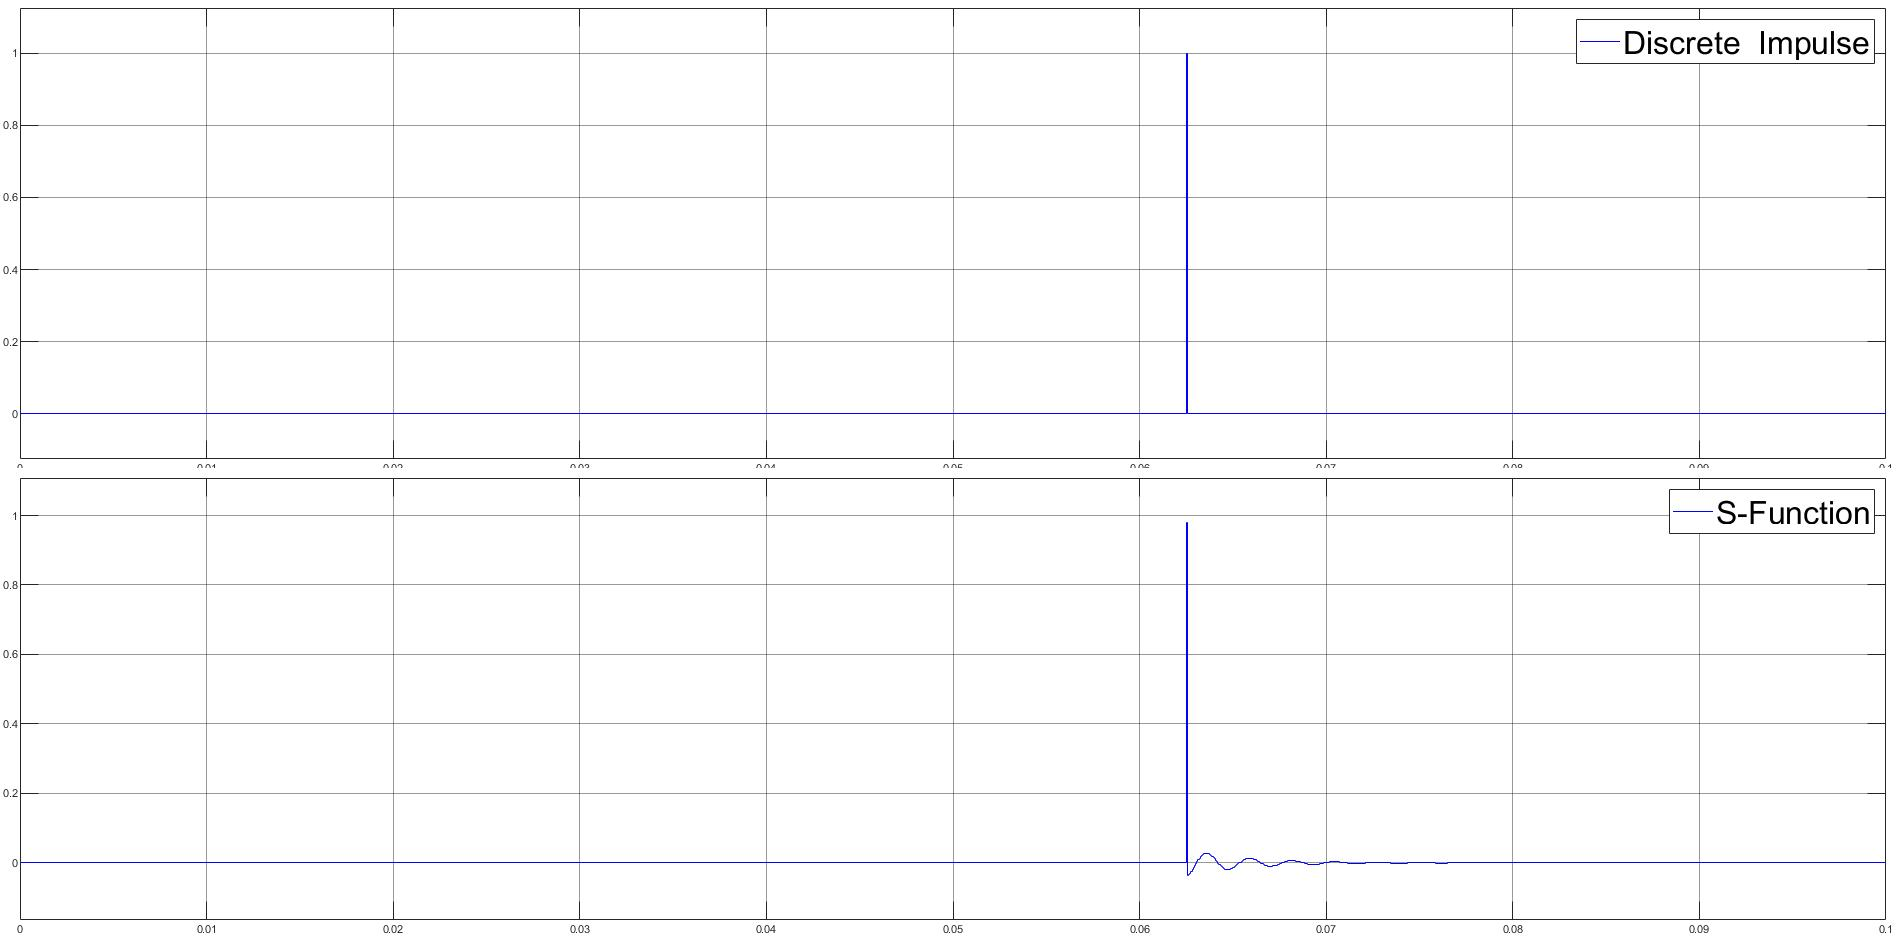
\includegraphics[scale = 0.2]{Figuras/p6_1-Impulse_100.jpg}
    \caption{Gráfica en el tiempo en segundos de la respuesta impulso del filtro diseñado con ancho de banda de $100~Hz$.}
    \label{impbw100}
\end{figure}

\begin{figure}[H]
    \centering
    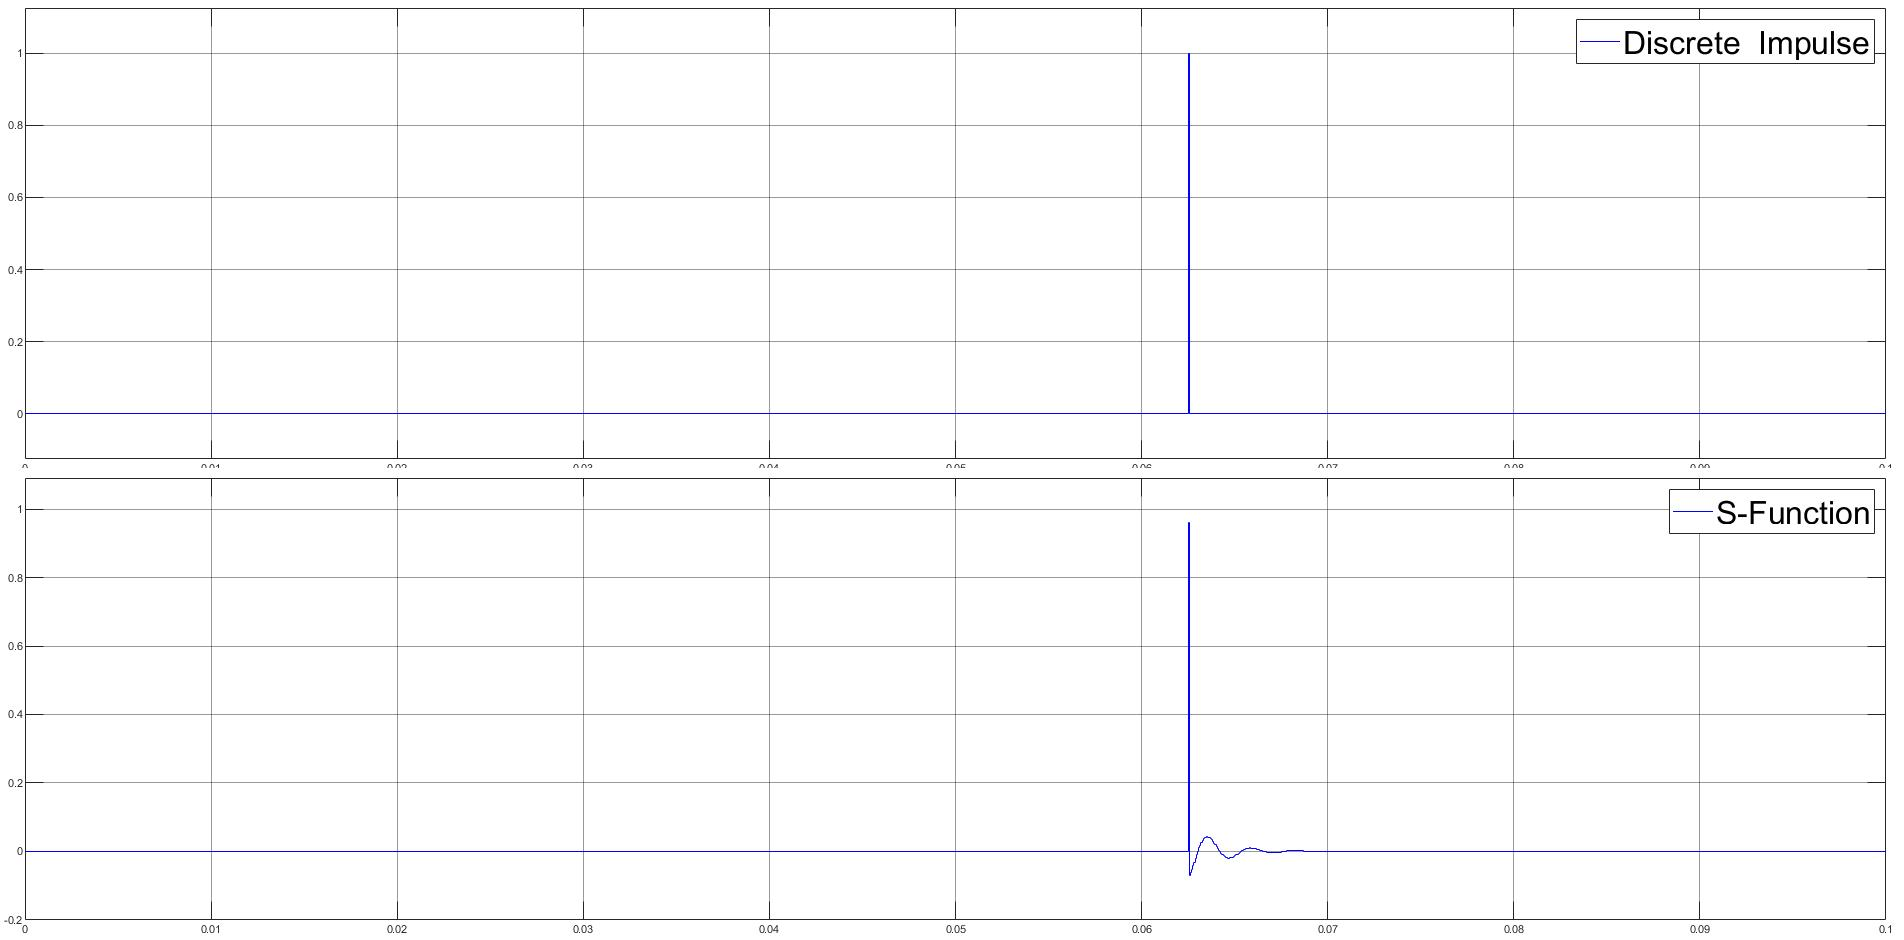
\includegraphics[scale = 0.2]{Figuras/p6_1-Impulse_200.jpg}
    \caption{Gráfica en el tiempo en segundos de la respuesta impulso del filtro diseñado con ancho de banda de $200~Hz$.}
    \label{impbw200}
\end{figure}


En las tres gráficas anteriores se puede comprobar lo antes mencionado sobre la relación inversa que existe entre la duración de la respuesta temporal del filtro con el ancho de banda permitido por este.

%Rodrigo
\item En esta sección se implementa filtro notch (elimina banda angosta) de segundo orden cuya frecuencia central pueda ser sintonizada en tiempo real. Para lo anterior se creó la función \texttt{filterInterface()} en C, la cual actualiza los parámetros del filtro, llama a la función \texttt{filterBiquad()} y actualiza la salida.

La primera parte de la sección de actualización de parámetros del filtro se muestra a continuación:\clearpage
\begin{lstlisting}[language = C]
void filterInterface(double input1, double input2,
                     double* output1) {

    //Calculo parámetros filtro
    double BW    = 2 * PI * 100 / 16000;    // (BW Norm)
    double theta = 2 * PI * input2 / 16000; // (wc Norm)

    double p[] = { cos(BW), -2, cos(BW) };
    double d1 = (-p[2] + sqrt(p[2] * p[2] - 4 * p[1] * p[3])) 
                / 2 * p[1];
    double d2 = (-p[2] - sqrt(p[2] * p[2] - 4 * p[1] * p[3])) 
                / 2 * p[1];

    double d;
    if (abs(d1) < abs(d2)) {
        d = d1;
    }
    else {
        d = d2;
    }
\end{lstlisting}
donde se utiliza la expresión de la solución de la ecuación cuadrática característica del filtro notch (\ref{p4_cuadratica}) y se extrae la extrae la solución que está dentro del círculo unitario por estabilidad.

La segunda parte de la sección de actualización de parámetros del filtro se muestra a continuación:
\begin{lstlisting}[language = C]
    //Actualizacion de parametros filtro
    static bqState_t Notch_variable = {
                      0,  // a1
                      0, // a2
                      0, //b0
                      0,//b1
                      0,  //b2

                      {0, 0, 0}, //Inputs buffer
                      {0, 0, 0} //Outputs buffer
    };

    (&Notch_variable)->bqA1 = -(1 + d) * cos(theta);
    (&Notch_variable)->bqA2 = d;
    (&Notch_variable)->bqB0 = (1 + d) / 2;
    (&Notch_variable)->bqB1 = (1 + d) / 2 * -2 * cos(theta);
    (&Notch_variable)->bqB2 = (1 + d) / 2;

\end{lstlisting}
donde se utiliza la función de transferencia dependiente de $d$ (\ref{p6_Transfer}) para obtener los coeficientes $a_i$ y $b_i$.

Finalmente se llama a la función \texttt{filterBiquad()} como se muestra a continuación con el filtro ya actualizado.
\begin{lstlisting}[language = C]
//Llamado a funcion de filtrado y seteo de salida
    *output1 = filterBiquad(&Notch_variable, input1);
}
\end{lstlisting}
Ya con \texttt{filterInterface()} implementada, se genera la función para crear la s-Function:

\begin{lstlisting}[language = C]
extern double notch(double data1, double data2)
{
    double output;
    filterInterface(data1, data2, &output);
    return output;
}
\end{lstlisting}

Posteriormente se creó un diagrama en simulink para probar la s-Function. Dicho diagrama se muestra en la figura \ref{fig:p6_2_simulink}. Aquí se ocupo el bloque \textit{Repeating Sequence Interpolated} para generar la señal de control de frecuencia central, donde la señal se mantiene en 440 Hz el primer segundo, luego aumenta a razón constante hasta el segundo 3 donde se queda en 880 Hz hasta los 3.9 s (donde se termina la simulación). 
\begin{figure}[H]
    \centering
    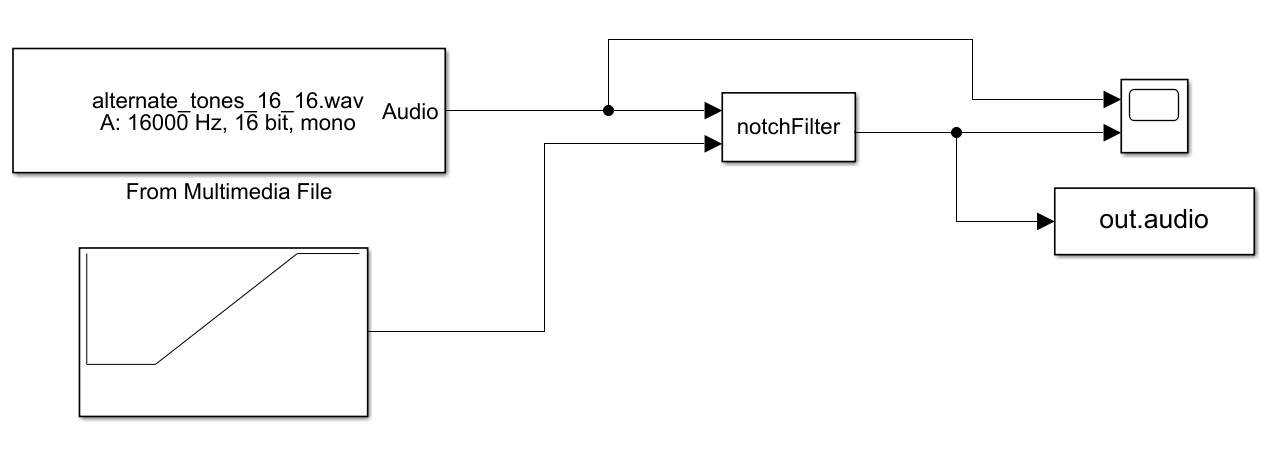
\includegraphics[width = .8\linewidth]{Figuras/p6_2_simulink.png}
    \caption{Diagrama en simulink para el testeo de la s-Function de notch ajustable}
    \label{fig:p6_2_simulink}
\end{figure}
 
 La señal de  audio a filtrar(\textit{alternate\_tones\_16\_16.wav}) y la filtrada se muestra en la figura \ref{fig:p6_2_scope}. Se observa que durante el primer segundo se filtra la primera señal en 440 Hz, que a partir del segundo 3 se filtra la segunda en 880 Hz y que existe una transición entre el segundo 1 y 3. Resulta interesante destacar que el filtro también afecta la amplitud de la señal que se desea dejar pasar. 
 
 \begin{figure}[H]
    \centering
    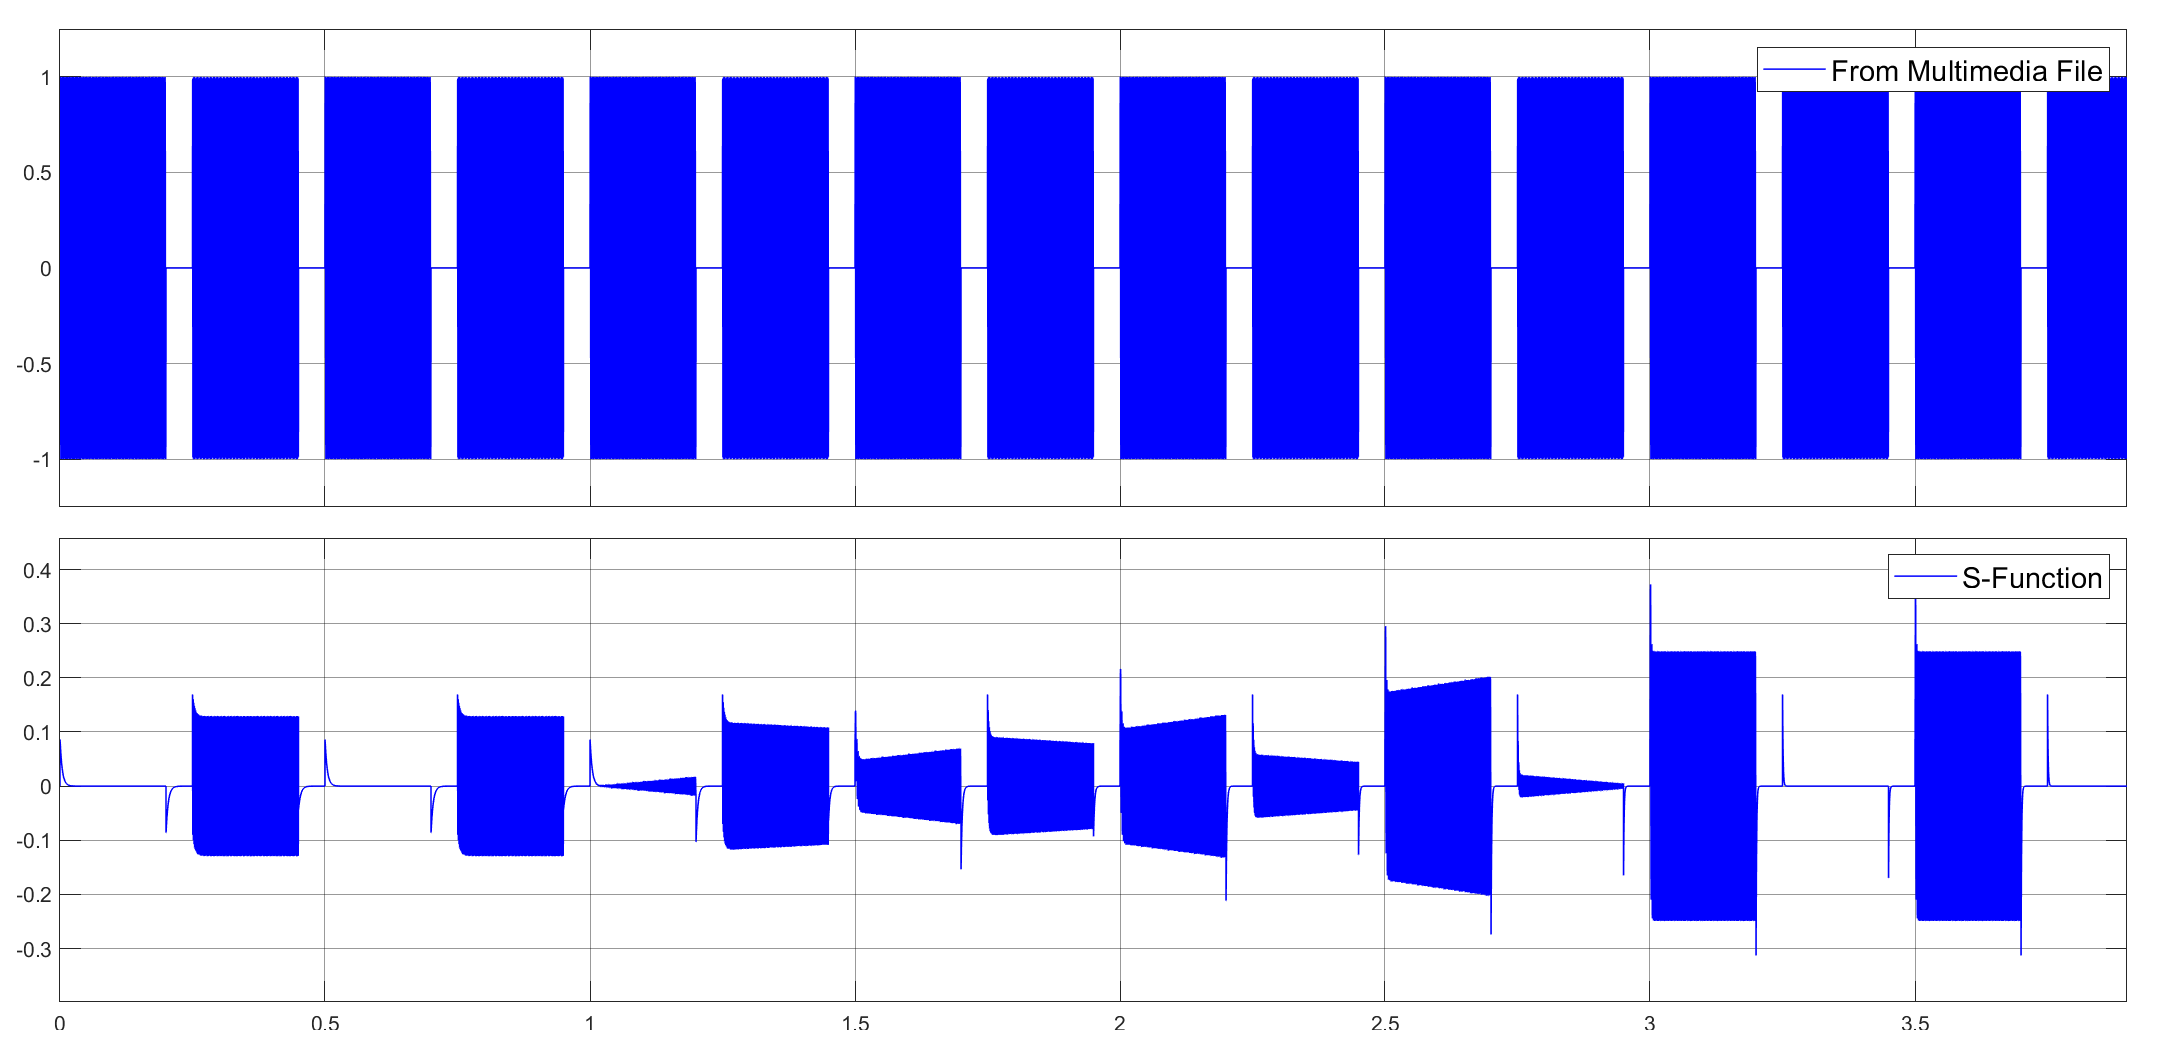
\includegraphics[width = .8\linewidth]{Figuras/p6_2_scope.eps}
    \caption{Amplitud [-] vs tiempo [s] de señal de entrada al filtro notch ajustable (arriba) y señal resultante del filtrado (abajo).}
    \label{fig:p6_2_scope}
\end{figure}

La señal de salida se guarda en el archivo de audio \texttt{p6\_2\_alternate\_audio\_16.wav} el cual se adjunta en la entrega. Auditívamente se aprecia correcto funcionamiento del esquema (no percepción de la frecuencia baja al inicio y solo percepción de la frecuencia alta al final).

%Richi
\item  Se diseñan 7 filtros pasa banda angosta para poder identificar tonos dtmf presentes en el archivo de audio \textit{dtmf\_secuence.wav}. Para esto se deben escoger los coeficientes $a_k$ y $b_k$ asociados a la función de transferencia de la forma de un filtro Biquad que se ha estado utilizando, de manera que cada filtro permita pasar una des las frecuencias de los tonos dtmf es decir

$$BPF0: ~~ 696~Hz $$
$$BPF1: ~~ 770~Hz  $$
$$BPF2: ~~ 852~Hz  $$
$$BPF3: ~~ 941~Hz  $$ 
$$BPF4: ~~ 1209~Hz  $$ 
$$BPF5: ~~ 1336~Hz  $$
$$BPF6: ~~ 1447~Hz  $$


Se desarrolló un script en MATLAB que permite obtener los coeficientes necesarios para filtrar cada una de las frecuencias dado un ancho de banda y  una frecuencia de muestreo. Se escogió un ancho de banda de $20~Hz$, ya que es un valor que permite aislar completamente cada frecuencia deseada asegurando que no aparezcan componentes de otras frecuencias que no le corresponden al filtro asociado. Se hicieron pruebas con anchos de banda mas holgados considerando las consecuencias en la respuesta temporal que este parámetro implica (un ancho de banda mayor genera una respuesta transciente menor) pero no se logró filtrar de manera precisa la frecuencias de interés.

El cuadro \ref{coeficientes} muestra los coeficientes $a_k$ y $b_k$ correspondientes a cada filtro asociado a una frecuencia específica


 
 \begin{table}[H]
        \centering
        \begin{tabular}{|c|c|c|c|c|c|}
        \hline
         Frecuencia [Hz]   & a_1 & a_2 & b_0 & b_1 & b_2\\
         \hline
         697  &  -1.91801  & 0.99217 &  0.00391             &      0&  -0.00391 \\
         \hline
         770  & -1.90179 &  0.99217 & 0.00391          &        0  &-0.00391	 \\
         \hline
         852 &   -1.88170 &  0.99217 & 0.00391       &          0 & -0.00391\\
         \hline
        
         941  & -1.85769 &  0.99217 &  0.00391      &          0 & -0.00391\\
         \hline
        
        1209  &  -1.77183 &  0.99217&	  0.00391         &      0 & -0.00391\\
         \hline
        
         1336  & 	-1.72423 &  0.99217  & 0.00391     &             0 & -0.00391\\
         \hline
         
        1447  &  -1.66636 &  0.99217 &  0.00391     &             0&  -0.00391	\\
         \hline

        \end{tabular}
        \caption{Cuadro resumen de los coeficientes de $a_k$ y $b_k$ de los filtros asociados a cada frecuencia dtmf.}
        \label{coeficientes}
    \end{table}
    
    
    Para implementar los filtros se creó para cada uno  estructura del tipo \texttt{bqState\_t} como la que se ha estado usando hasta el momento con los coeficientes asociados a cada uno de los mismos, se reutiliza la función \texttt{filterBiquad} ya implementada y se desarrolla la función \texttt{decodeDtmf} que llama a las funciones entregadas como recurso para el laboraorio para poder ejecutar la decodificación que se busca. El código de la función \texttt{decodeDtmf} es el siguiente
    
    \begin{lstlisting}[language = C]
extern  void decodeDtmf(double input1, int32_t *output1){
  gDtmfTones[0] = filterBiquad(&BPF0,input1);
  gDtmfTones[1] = filterBiquad(&BPF1,input1);
  gDtmfTones[2] = filterBiquad(&BPF2,input1);
  gDtmfTones[3] = filterBiquad(&BPF3,input1);
  gDtmfTones[4] = filterBiquad(&BPF4,input1);
  gDtmfTones[5] = filterBiquad(&BPF5,input1);
  gDtmfTones[6] = filterBiquad(&BPF6,input1);

  *output1 =   dtmfDetection(gDtmfTones);
}
    \end{lstlisting}


Al simular el filtrado de la señal de audio \textit{dtmf\_secuence.wav} con los filtros implementados se obtiene la gráfica que se muestra en la figura \ref{dtmf}

\begin{figure}[H]
    \centering
    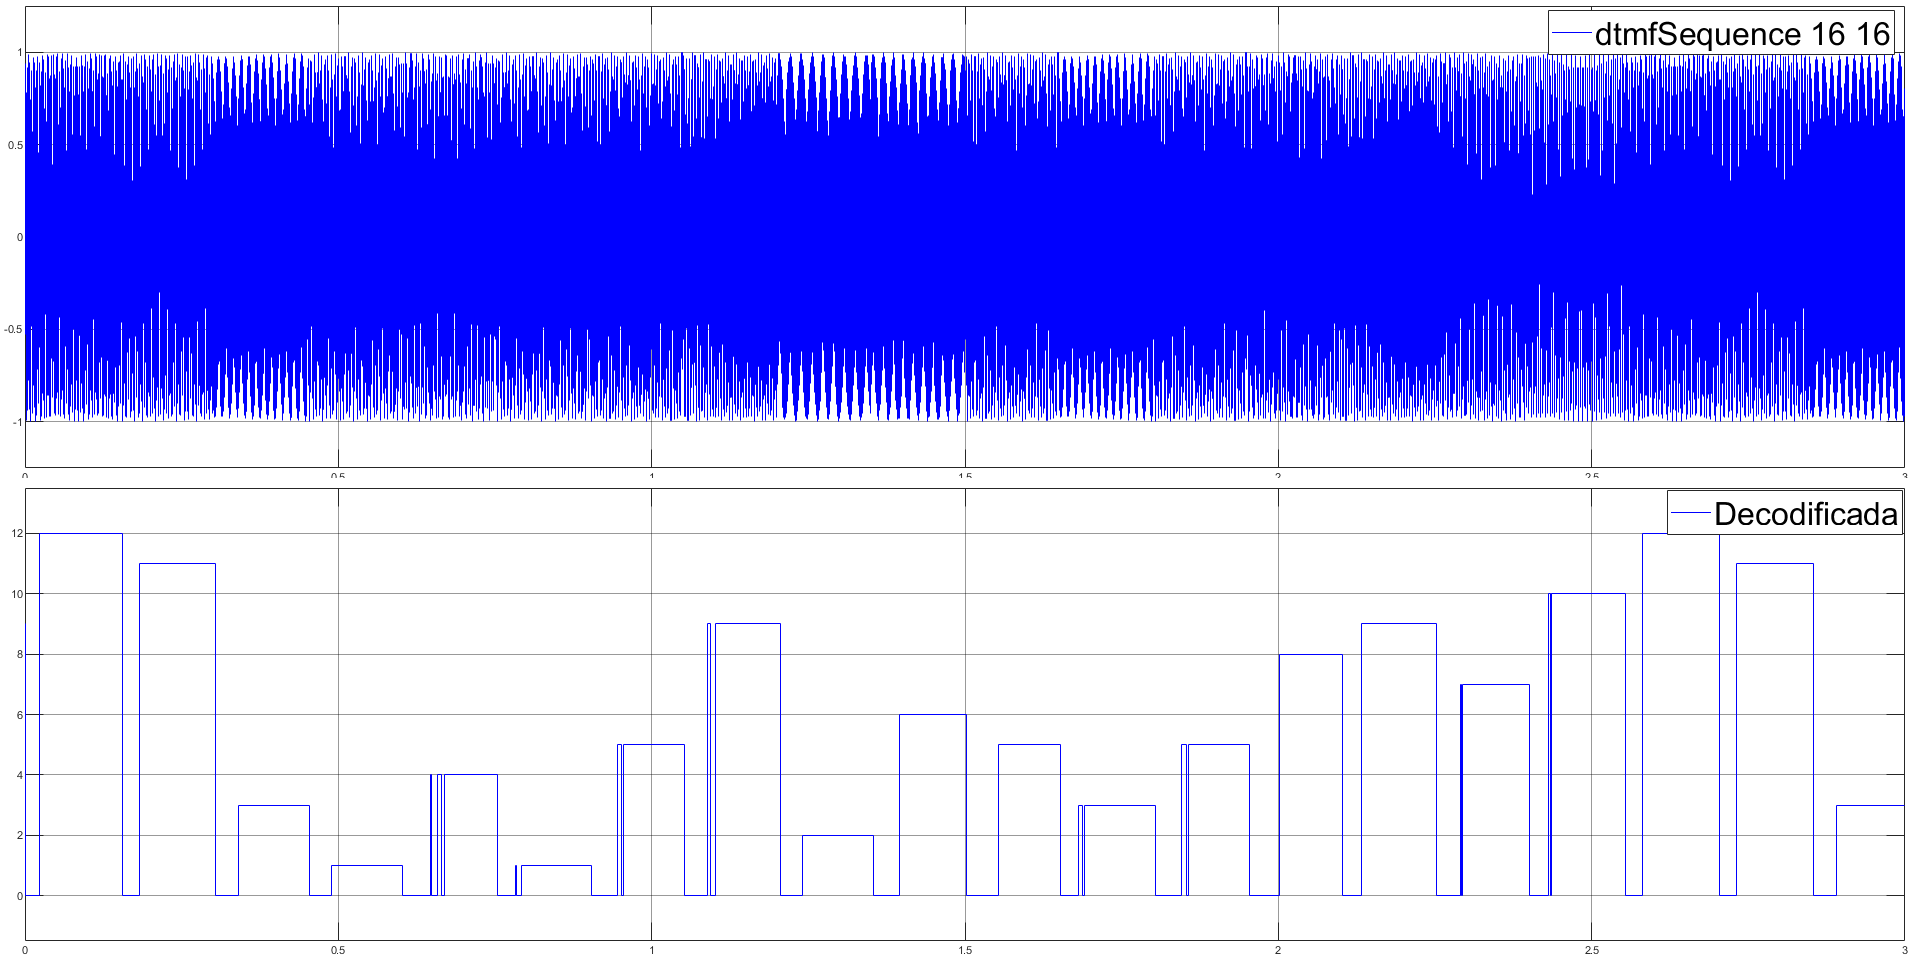
\includegraphics[scale = 0.3]{Figuras/p6_3-Dtmf.png}
    \caption{Gráfica en el tiempo en segundos de la simulación de filtrado de la señal de audio \textit{dtmf\_secuence.wav} con 7 filtros BPF  en paralelo.}
    \label{dtmf}
\end{figure}


La gráfica superior muestra el archivo de audio en el tiempo  y la gráfica inferior muestra el resultado obtenido luego de filtrar la señal, donde se puede reconocer  la secuencia dtmf era \texttt{\#-*-3-1-4-1-5-9-2-6-5... - \#}.

\end{enumerate}